\documentclass[compsoc]{IEEEtran}
\usepackage{graphicx}
\usepackage{amsmath}
\usepackage{authblk}
\usepackage[english]{babel}
\usepackage{blindtext}
\usepackage[ruled,vlined,linesnumbered]{algorithm2e}
\usepackage{algorithmic,float}
\usepackage{setspace}
\usepackage{amsfonts}
\usepackage{hyperref}
\graphicspath{ {./images/} }
\usepackage{fontspec}
\usepackage{listings}
\usepackage{amsmath}
\usepackage{mathabx}
\newfontfamily\listingsfont[Scale=.7]{Ubuntu}\usepackage[font=footnotesize,labelfont=bf]{caption}
\usepackage[table,xcdraw]{xcolor}
\usepackage[utf8]{inputenc}
\title{Parallelization of the Floyd-Warshall algorithm}
\author{David Bertoldi -- 735213 \\ email: d.bertoldi@campus.unimib.it}
\affil{Department of Informatics, Systems and Communication}
\affil{University of Milano-Bicocca}
\date{June 2020}

\definecolor{mGreen}{rgb}{0,0.6,0}
\definecolor{mGray}{rgb}{0.5,0.5,0.5}
\definecolor{mPurple}{rgb}{0.58,0,0.82}
\definecolor{backgroundColour}{rgb}{0.95,0.95,0.92}

\lstdefinestyle{CStyle}{
    backgroundcolor=\color{backgroundColour},   
    commentstyle=\color{mGreen},
    keywordstyle=\color{magenta},
    numberstyle=\tiny\color{mGray},
    stringstyle=\color{mPurple},
    basicstyle=\linespread{1}\listingsfont,
    breakatwhitespace=false,         
    breaklines=true,                 
    captionpos=b,                    
    keepspaces=true,                 
    numbers=none,                    
    numbersep=5pt,                  
    showspaces=false,                
    showstringspaces=false,
    showtabs=false,                  
    tabsize=2,
    language=C,
}

\begin{document}

\maketitle 



\begin{abstract}
The well known Floyd-Warshall (FW) algorithm solves the all-pairs shortest path problem on directed graphs. In this work we parallelize the FW using three different
programming environments, namely MPI, OpenMP and CUDA. We experimented with multiple data sizes, in order to gain insight on the execution behavior
of the parallelized algorithms on modern multicore and distributed platforms, and on the programmability of the aforementioned environments. We were able
to significantly accelerate FW performance utilizing the full capacity provided by the architectures used.
\end{abstract}

todo: descrizione openmp, cude, mpiP, wakeupGPU


\section{Introduction and Background}
The FW is a classic dynamic programming algorithm that solves the \emph{all-pairs shortest path (APSP)} problem on directed weighted
graphs $G(V, E, w)$, where $V = \{1, \dots, n\}$ is a set of nodes, $E \subseteq V \times V$ are the edges and $w$ is a weight function $E \rightarrow  \mathbb{R}$
that expresses the cost of crossing two nodes. The number of nodes is denoted by $n$ and the number of edges by $m$ . \par
The output of the algorithm is typically in matrix form: the entry in the $i$th row and $j$th column is the weight of the shortest path between
nodes $i$ and $j$. FW runs in $\Theta(|V|^3)$ time and for this reason is a good choiche when working with dense graph: even though there
may be up to $\Omega(|E|^2)$ edges, the computational time is independent from the number of edges. \par
The FW algorithm is shown in \textbf{Algorithm \ref*{alg:fw1}}.

\begin{algorithm}[h!]

\SetAlgoLined

\For{$(u, v) \in E$}{
    $M_{u, v} \leftarrow w(u, v)$
}
\For{$v = 1 \rightarrow n$}{
    $M_{v, v} \leftarrow 0$
}
 \For{$k = 1 \rightarrow n$}{
  \For{$i = 1 \rightarrow n$}{
  \For{$j = 1 \rightarrow n$}{
  \If{$M_{i, j} > M_{i, k} + M_{k, j}$}{
 
    $M_{i, j} \leftarrow M_{i, k} + M_{k, j}$ 
 }
 }
 }
 }
 
\caption{The Floyd-Warshall (FW) algorithm}\label{alg:fw1}
\end{algorithm}

A C implementation of this algorithm can be found \href{https://github.com/firaja/Parallel-FloydWarshall/blob/master/sequential.c}{here};
this version is referred in this document as \emph{sequential} implementation and it is used as base version when comparing to parallel implementations. \par 

\section{Methodology}
\subsection{Strategy}
It's easy to notice that the nested $i$ and $j$ for-loops in \textbf{Algorithm \ref*{alg:fw1}} can be parallizable, but one of the \emph{intermediate edges} for a process
could be the \emph{edge under analysis} for another process. For example process $P^1$ is writing in a cell while process $P^2$ is reading from the same cell, leading to a unpredictable final result
if $P^1$'s writing comes before or after $P^2$'s reading.

It seems that enabling parallelization requires some sort of blocking mechanism between processes, like a semaphore, but we prove that no data race can occur as in the previous example as far as $k$
is shared between processes. 

Let's assume we have 2 processes, namely $P^1$ and $P^2$ and they have \emph{under analisys} $M_{i,j}$ and $M_{x,y}$ respectively, with $x \neq i$. 
At any point the following system of preconditions exists (the two inequalities are taken from \textbf{Algorithm \ref*{alg:fw1}} at line 10):

\begin{flalign}\label{eq:sys1}
 &&  \left\{\begin{matrix}
P^{1}_{i,j} & > & P^{1}_{i,k} & + & P^{1}_{k,j} \\
\\ 
P^{2}_{x,y} & > & P^{2}_{x,k} & + & P^{2}_{k,y}
\end{matrix}\right. &&
\end{flalign}

\emph{i.e.} $P^1$ is reading values of $M_{i,k}$ and $M_{k,j}$ so it can decide if $M_{i,j}$ should be overwritten; 
the same does $P^2$ with $M_{x,k}$, $M_{k,y}$ and $M_{x,y}$ respectively. \\
In order to have a data race, the following must be true as well

\[(x = i \wedge k=j) \vee (k = i \wedge y = j)\]

\emph{i.e.} $P^2$ is using as one of its \emph{intermediate edges} the \emph{edge under analysis} of $P^1$. Without losing
of generality we do not analyze the opposite case because the proof develops symmetrically.\\
Because $x \neq i$, only the following must be verified

\begin{flalign}\label{eq:cond1}
 &&  k = i \wedge y = j &&
\end{flalign}
and by applying (\ref*{eq:cond1}) to (\ref*{eq:sys1}) we have

\begin{flalign}\label{eq:sys2}
 &&  P^{1}_{i,j} > P^{1}_{k,k} + P^{1}_{i,j} &&
\end{flalign}
but (\ref*{eq:sys2}) is clearly false, because $M$ is a hollow matrix \emph{i.e.} the  diagonal elements are all equal to $0$, leaving the 
following inequality:
\begin{flalign}\label{eq:sys3}
 &&  P^{1}_{i,j} > P^{1}_{i,j} &&
\end{flalign}
Clearly no number can be greater than itself and this means that at this point the comparison made by $P^1$ is irrilevant
and is always evalueted false. If $P^2$ writes after or before $P^1$'s evaluation does not really matter and thus 
there is no data race as far as $k$ is the same for all the processes.

This is really important because it assures that there is no need for locking mechanism on $M$ when it comes to
parallelize the nested $i$ and $j$ for-loops and having no blocks guarantees better performance.

So the strategy relies on dividing the matrix by rows and assigning an equal number of rows to each process.
Once $k$ is set and it's shared among all processes, each process puts \emph{under analysis} every cell
of its sub-matrix and selects its \emph{intermediate edges} depending on $k$.

In this work we propose 3 parallel architectures implemented with 3 different parallel programming environments: 
\emph{Distributed computing} with MPI, \emph{Mutithreading} with OpenMP and \emph{GPGPU} with CUDA.

The document analyzes each implementation and gives an overview of timings, implementations and pros and cons for each case.

\subsection{Distributed with MPI}

Message Passing Interface (MPI) is a standardized and portable message-passing standard designed by a group of researchers from academia and industry to function on a wide variety of parallel computing architectures. The standard defines the syntax and semantics of a core of library routines useful to a wide range of users writing portable message-passing programs in C, C++, and Fortran. There are several well-tested and efficient implementations of MPI, many of which are open-source or in the public domain. These fostered the development of a parallel software industry, and encouraged development of portable and scalable large-scale parallel applications. \par

The main strategy is based on scattering horizontally the whole matrix among all the process, so that
each process can read a portion of the matrix of size $\frac{n^2}{p}$; then a \emph{process of competence}
is chosen: as $k$ is in common (but never transmitted) to all the processes, there's always a cell in the $k$th
row representing one of the two intermediate vertices for any process and there's always one process to which this row was assigned.
The value $k$ is always "synchronized" between process because each for-loop involving $k$ starts with a collective communication
which implies a synchronization point among processes.

\begin{figure}[h!]
\centering                                                                        
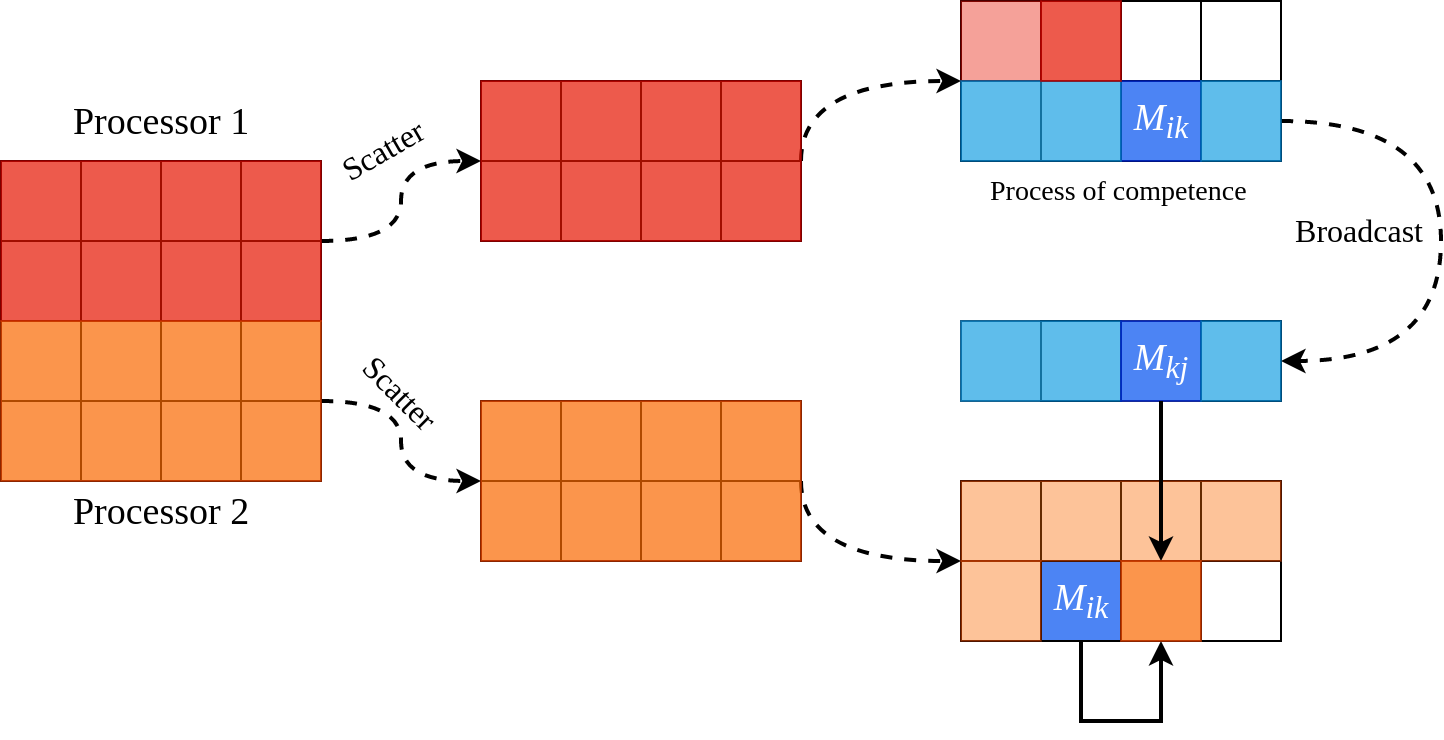
\includegraphics[width=3.5in]{diagrams/mpi-scatter}
\captionsetup{justification=centering}                                                                                                                                   
\caption{View of the data each thread can reach}                                                                                                                                            
\label{fig:threads}                                                                                                                                                           
\end{figure}
Everytime $k$ changes, the $k$th row is broadcasted to the other processes by the process that owns the row;
a total of $k$ \texttt{MPI\_Bcast} operations are required. \par
Once the $k$th row has been received, each process acts like the original FW in the $i$ and $j$ for-loops; obviously
they each write values in their own local matrix. \par

At the end of the $k$ for-loop, all the local matrices are gathered to the root process. 
\textbf{Algorithm \ref*{alg:mpi}} shows an high level implementation of the strategy exposed above.\par

\begin{algorithm}[h!]

\SetAlgoLined

broadcast($n$, $ROOT$) \\
scatter($M$, $processes$)

\For{$k = 1 \rightarrow n$}{
	\If{$rank =$ \textnormal{findOwnerOfKthRow}($k$, $rank$)}{
		$K \leftarrow $ getRow($M$, $k$) \\
		broadcast($K$, $owner$) \\
	}
	\For{$i = 1 \rightarrow \frac{n}{processes}$}{
		\For{$j = 1 \rightarrow n$}{
			\If{$M_{i,j} < M_{i,k} + K_j$}{
				$M_{i,j} \leftarrow M_{i,k} + K_j$
			}
		}
	}
}
gather($M$, $processes$);
 
\caption{Distributed version of FW}\label{alg:mpi}
\end{algorithm}


We can list all the communication required:
\begin{itemize}
\item{1 \texttt{MPI\_Bcast} for communicating the value of $n$}
\item{1 \texttt{MPI\_Scatter} for the assignment of the local sub-matrix}
\item{$k$ \texttt{MPI\_Bcast} for communicating the $k$th row}
\item{1 \texttt{MPI\_Gather} for the collection of the local sub-matrix}
\end{itemize}

\textbf{Table \ref*{tab:comm}} approximates how many bytes are involved in the communications, assuming that
the implementation uses 4 bytes to store one \texttt{int} and omitting the overhead of the communication protocol.
\begin{table}[h!]
\centering
\begin{tabular}{|l|l|l|}
\hline
\rowcolor[HTML]{F56B00} 
{\color[HTML]{FFFFFF} \textbf{Count}} & {\color[HTML]{FFFFFF} \textbf{Type}} & {\color[HTML]{FFFFFF} \textbf{Size}} \\ \hline
1                                     &  \texttt{MPI\_Bcast}                 &  $4(p-1)$ bytes                      \\ \hline
1                                     &  \texttt{MPI\_Scatter}               &  $4\frac{n^2(p-1)}{p}$ bytes         \\ \hline
$k = n$                               &  \texttt{MPI\_Bcast}                 &  $4n^2(p-1)$ bytes                    \\ \hline
1                                     &  \texttt{MPI\_Gather}                &  $4\frac{n^2(p-1)}{p}$ bytes         \\ \hline
\end{tabular}
\caption{Execution time of the \emph{MPI} FW}                                                                                                                                            
\label{tab:comm}
\end{table}
\par

Total communications can be expressed with the following formula, that can help to calculate the bandwidth of the network
for this implementation:
\[W_{comm} = 4(p-1)(1 + n^2(1 + \frac{2}{p})) \text{ bytes}\]
This formula is important because the time spent on communications is time taken from the calculation and a network with an inadequate
bandwith is the main source of bottlenecks. For example having 8 processes consuming a $12500 \times 12500$ matrix implies a total of
$\textasciitilde 5.46$GB transferred  over the entire network; this means that each processor would theorically spend $5468$ms (43 seconds in total) on communication over a 1Gbps network.

\begin{figure}[h!]
\centering                                                                        
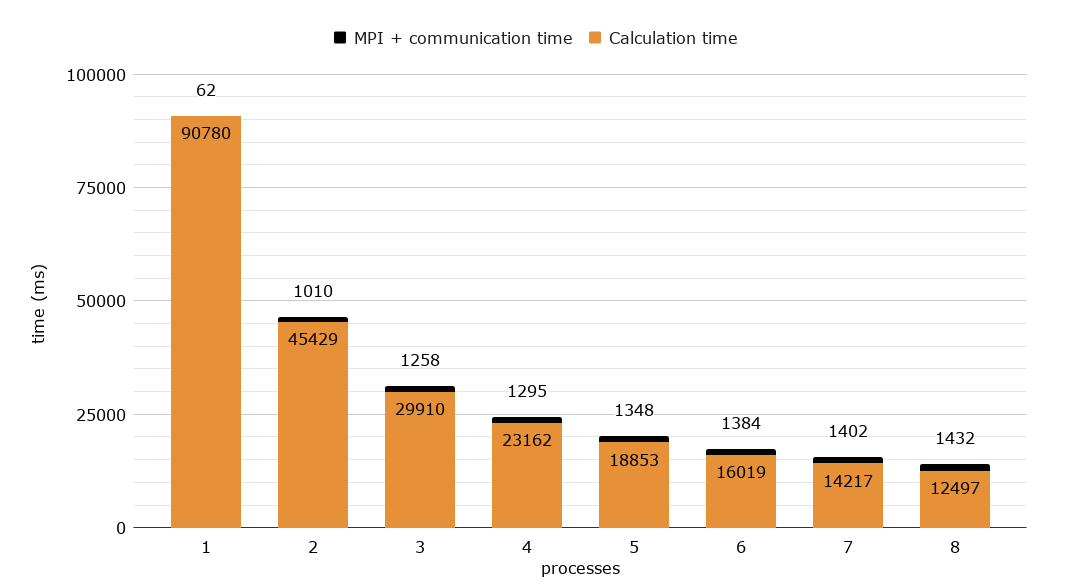
\includegraphics[width=3.5in]{diagrams/mpi-time}
\captionsetup{justification=centering}                                                                                                                                   
\caption{Calculation and MPI instantiation + communication time of \emph{MPI} FW consuming a $5040\times5040$ matrix over a 1Gbps network depending on the number of processes}
\label{fig:mpi-time}                                                                                                                                                           
\end{figure}

\textbf{Figure \ref*{fig:mpi-time}} shows the amount of time taken to initialize the MPI cluster and communicate during the execution of the \emph{MPI} FW. In this case a dense 
$5040\times5040$ matrix is used for input and the MPI cluster was located in a star network with 1Gbps bandwith.

The overhead has a quadratic or linear growth with respect to the number of vertices and or the number of processes respectively; 
so with a medium-small matrix the time used in communication can exceed the 10\% of the total computational time. 
But by increasing the size of the matrix to $12600\times12600$ the time used in communication drops to 4\%, with a total of 50 seconds. Thus the implementation fits well for huge matrixes, rather than medium ones.

For this reason the speedup is considerable but far from the ideal for a $5040\times5040$ matrix. \textbf{Figure \ref*{fig:mpi-speedup}} shows the trend of the speedup in relation to the 
sequential version.

\begin{figure}[h!]
\centering                                                                        
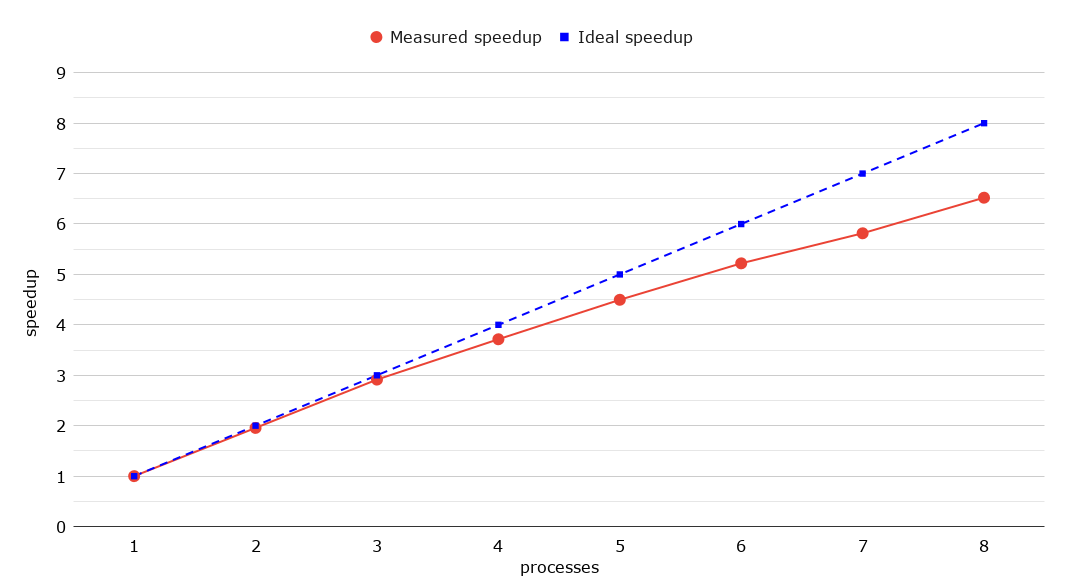
\includegraphics[width=3.5in]{diagrams/mpi-speedup}
\captionsetup{justification=centering}                                                                                                                                   
\caption{Speedup of \emph{MPI} FW}                                                                                                                                            
\label{fig:mpi-speedup}                                                                                                                                                           
\end{figure}

With a consequent decrease in efficiency as shown in \textbf{Figure \ref*{fig:mpi-efficiency}}
\begin{figure}[h!]
\centering                                                                        
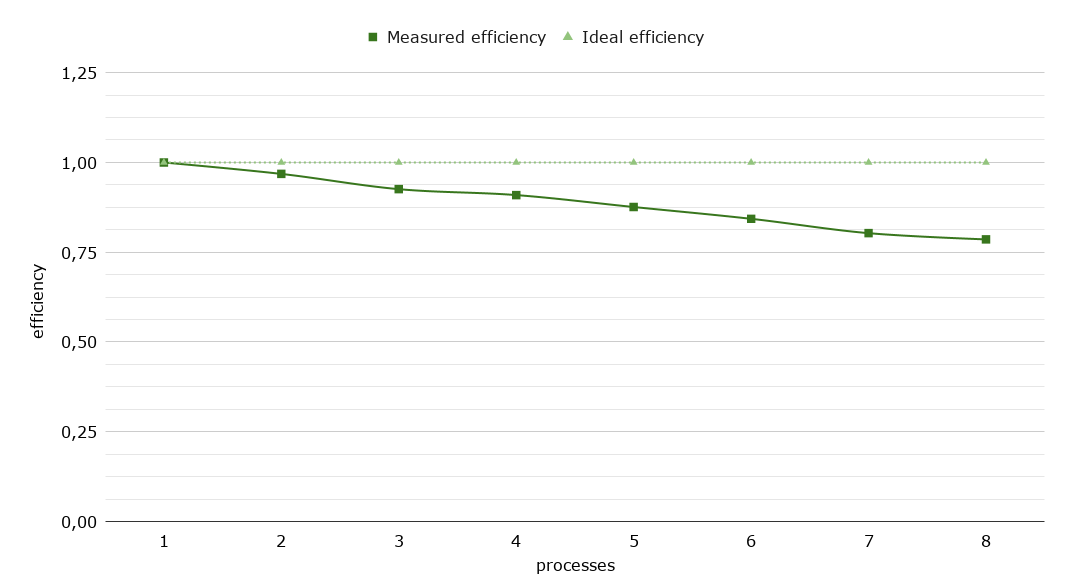
\includegraphics[width=3.5in]{diagrams/mpi-efficiency}
\captionsetup{justification=centering}                                                                                                                                   
\caption{Efficiency of \emph{MPI} FW consuming a medium matrix}                                                                                                                                            
\label{fig:mpi-efficiency}                                                                                                                                                           
\end{figure}























































\subsection{Multithreading with OpenMP}
OpenMP (Open Multi-Processing) is an application programming
interface (API) for parallel programming intended to work on shared-
memory architectures. More specifically, it is a set of compiler
directives, library routines and environmental variables, which in-
fluence run-time behavior. OpenMP enables parallel programming in
various languages, such as C, C++ and FORTRAN and runs on most
operating systems. \par
The OpenMP API uses the fork-join model of parallel execution.
Multiple threads perform tasks defined implicitly or explicitly by
OpenMP directives. All OpenMP applications begin as a single thread
of execution, called the initial thread. The initial thread executes
sequentially until it encounters a parallel construct. At that point,
this thread creates a group of itself and zero or more additional
threads and becomes the master thread of the new group. Each thread
executes the commands included in the parallel region, and their
execution may be differentiated, according to additional directives
provided by the programmer. At the end of the parallel region, all
threads are synchronized. \par
The runtime environment is responsible for effectively scheduling
threads. Each thread, receives a unique id, which differentiates it
during execution. Scheduling is performed according to memory
usage, machine load and other factors and may be adjusted by altering
environmental variables. In terms of memory usage, most variables in
OpenMP code are visible to all threads by default. However, OpenMP
provides a variety of options for data management, such as a thread-
private memory and private variables, as well as multiple ways of
passing values between sequential and parallel regions. Additionally,
recent OpenMP implementations introduced the concept of tasks,
as a solution for parallelizing applications that produce dynamic
workloads. Thus, OpenMP is enriched with a flexible model for
irregular parallelism, providing parallel while loops and recursive
data structures. \par
The main advantage on using OpenMP is the ease of developing parallelisms
with simple constructs that do not differ too much from the original implementation.

The snippet at \textbf{Algorithm \ref*{alg:omp}} shows the implementation used in this work: the matrix containing the
distances between vertices is shared among all the threads, while the 3 nested for-loops are executed
by each thread indipendentely.

\begin{algorithm}[h!]

\SetAlgoLined

\texttt{\#pragma omp parallel num\_threads(t) shared(M, k)} \\
\For{$k = 1 \rightarrow n$}{
	\texttt{\#pragma omp for private(i,j) schedule(dynamic)} \\
	\For{$i = 1 \rightarrow n$}{
		\For{$j = 1 \rightarrow n$}{
			\If{$M_{i,j} < M_{i,k} + K_j$)}{
				$M_{i,j} \leftarrow M_{i,k} + K_j$
			}
		}
	}
}

 
\caption{Multithreaded FW with \emph{OpenMP}}\label{alg:omp}
\end{algorithm}


Despite the overhead that the dynamic scheduler entails, in this case it works better than a static one because the
content of the sub-matrices varies from thread to thread so a group of threads may do more write operations on $M$ and a
static scheduler would make wait the others until they finish. 
 \\
Also note that the solution does not implement a \texttt{collapse} directive because when we collapse multiple loops, OpenMP turns them into a single loop: there is one
index that is constructed from \texttt{i} and \texttt{j} using division and modulo operations. This can
have huge impacts on the performance because of this overhead, especially if the matrix is really wide.

\textbf{Figure \ref*{fig:threads}} shows how 2 threads interact inside the matrix: the red and orange zones highlight the cells where
Thread 1 and Thread 2 can write respectively; the blue and turquise cells represent the intermediate vertices that are compared
with the vertice under analysis for Thread 1 and Thread 2 respectively.

\begin{figure}[h!]
\centering                                                                        
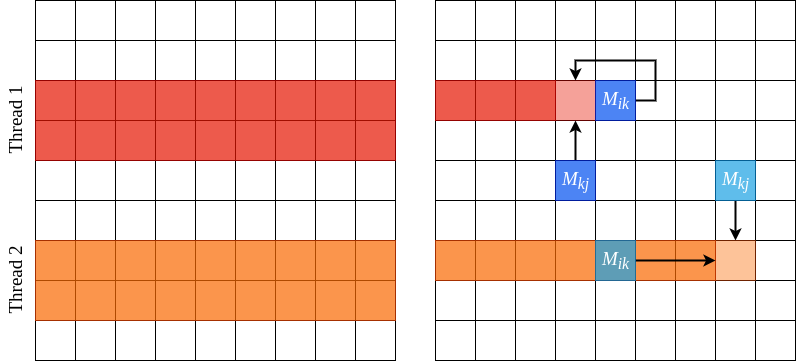
\includegraphics[width=3.5in]{diagrams/openmp-threads}
\captionsetup{justification=centering,margin=2cm}                                                                                                                                   
\caption{View of the data each thread can reach}                                                                                                                                            
\label{fig:threads}                                                                                                                                                           
\end{figure}


We prove that no race condition may appear in this case. 
No race condition can appear if $k$ is the same among the threads and threrfore there's no need to verify atomicity of the write operation;
the lack of OpenMP directive like \texttt{atomic} or \texttt{critical} plays in favor of performance. \par

The speedup of the solution is sligthy worse than the ideal speedup (see \textbf{Figure \ref*{fig:omp-speedup}})

\begin{figure}[h!]
\centering                                                                        
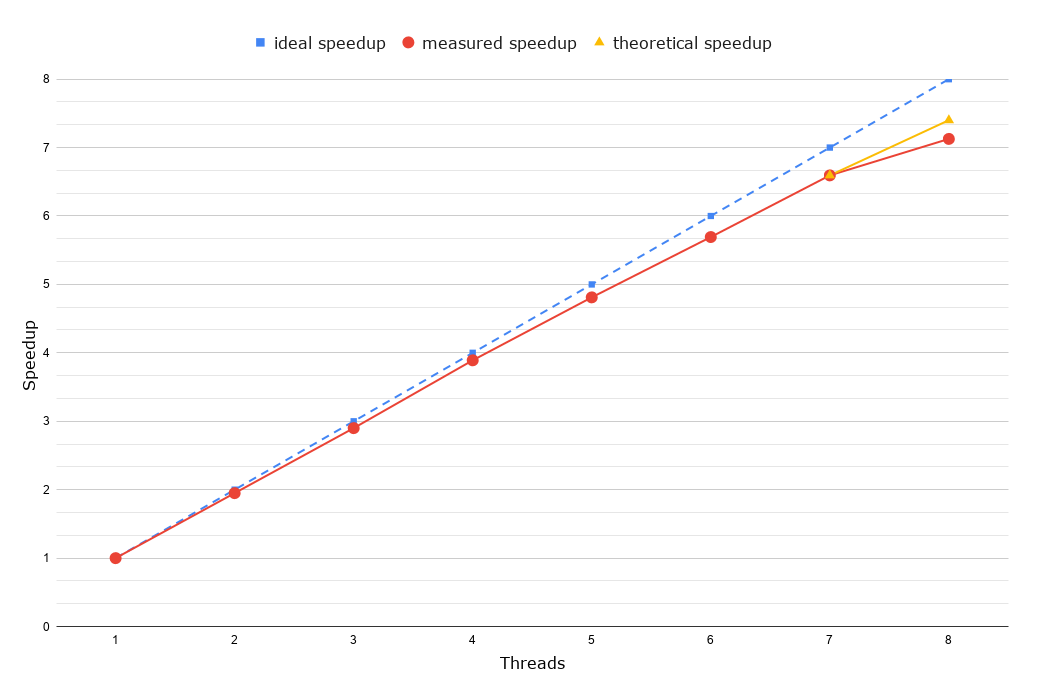
\includegraphics[width=3.5in]{diagrams/openmp-speedup}
\captionsetup{justification=centering,margin=2cm}                                                                                                                                   
\caption{Speedup of \emph{OpenMP} FW on a octacore CPU}                                                                                                                                            
\label{fig:omp-speedup}                                                                                                                                                           
\end{figure}
When scaling from 7 to 8 threads, we notice a slight deviation from the previous (almost) linear trend. That's because the measurement
is taken from a 8-core/8-thread CPU, namely Intel Core i7-9700K, and because no other cores were free to manage the OS and its subprocesses, the scheduler
divided this task among all the threads. So we have approximated the speedup without counting the fluctuations due to the management of the OS. \par

The efficiency, which stays always above $90\%$, is shown in \textbf{Figure \ref*{fig:omp-efficiency}} alongside with its theoretical counterpart.

\begin{figure}[h!]
\centering                                                                        
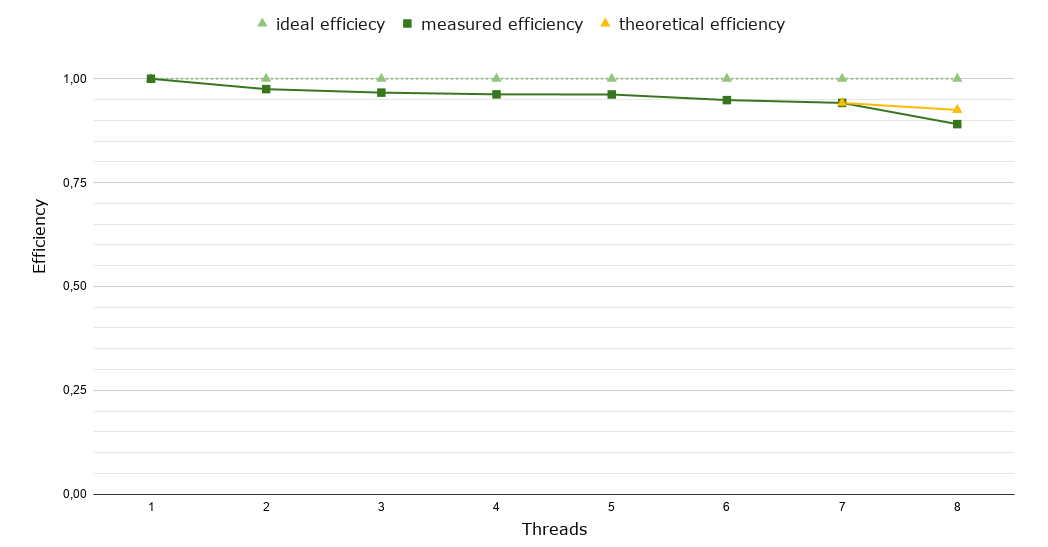
\includegraphics[width=3.5in]{diagrams/openmp-efficiency}
\captionsetup{justification=centering,margin=2cm}                                                                                                                                   
\caption{Efficiency of \emph{OpenMP} FW on a octacore CPU}                                                                                                                                            
\label{fig:omp-efficiency}                                                                                                                                                           
\end{figure}
An overview of the timings collected can be found in \textbf{Table \ref*{tab:omp-time}}.













































































\subsection{GPGPU with CUDA}
In recent years, many scientific and numeric GPGPU applications found success due to graphics hardware’s streaming data-parallel organizational model. 

The GPU serves, to an extent, as a coprocessor to the
CPU programmed through the CUDA API. A single program known as kernel is compiled to operate on the GPU
device to exploit the massive data parallelism inherit on Single Instruction, Multiple Data (SIMD) architecture. Groups
of threads then execute the kernel on the GPU. Threads
are organized into blocks which allow efficient sharing of
data through a high-speed shared memory region accessible to the programmer
directly through CUDA. Shared memory is shared among
threads in a block, facilitating higher bandwidth and overall
performance gains. Therefore, algorithms must intelligently
manage this fast shared memory cache effectively. This
will fully utilize the data parallelism capabilities of graphics
hardware and alleviates any memory latency that data intensive algorithms suffer from on the GPU.

Unlike the other two implementations, \emph{CUDA} FW can rely on its \emph{grid-of-blocks} system and thus the kernel can do no loops: $k$ is still shared among threads
so that no data race occurs but each thread instead of covering one or more rows, is assigned to a single cell. 



\begin{figure}[h!]
\centering                                                                        
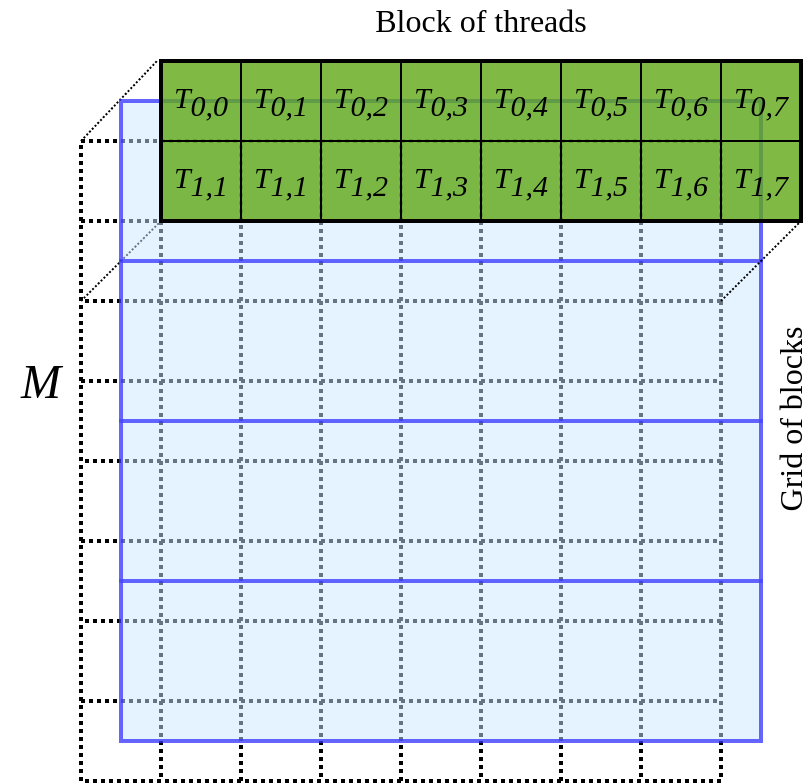
\includegraphics[width=2.5in]{diagrams/cuda-threads}
\captionsetup{justification=centering}                                                                                                                                   
\caption{Mapping of CUDA threads inside $M$}                                                                                                                                            
\label{fig:cuda-threads}                                                                                                                                                           
\end{figure}


Depending on the number of threads per block, each row  of matrix $M$ is covered by 1 or more blocks, that
have always height equal to 1 thread. This mapping allows threads of the same block share some data that can be reused. \\
In this case the shared variable stores the value $M_{i,k}$ that is in common with the entire row. Because the 
shared memory offers lower latency and higher bandwidth than the global memory, it is worth storing this value
for other threads.

\begin{algorithm}[h!]

\SetAlgoLined
\DontPrintSemicolon
  

\For{$k = 0 \rightarrow n$}{
	\textnormal{kernel<{}<{}<$\frac{n+b-1}{b} \times n$, $b$>{}>{}>($M$, $n$, $k$)}
}

\;

\SetKwFunction{FMain}{kernel}
  \SetKwProg{Fn}{Function}{:}{}
  \Fn{\FMain{$M$, $n$, $k$}}{

$j \leftarrow \left|B\right|_x \times B_x + T_x$ \\
$i \leftarrow \left|B\right|_y$ \\

\If{$j < n$}{
	
	\If{$T_x = 0 $}{
		$K_{\textnormal{shared}} \leftarrow M_{i,k};$
	}

	$\textnormal{syncthreads()}$


	\If{$M_{i,j} < K_{\textnormal{shared}} + M_{k,j}$}{
		$M_{i,j} \leftarrow K_{\textnormal{shared}} + M_{k,j}$
	}
}
}
 
\caption{Kernel of the \emph{CUDA-FW} on a pre-Fermi architecture}\label{alg:cuda}
\end{algorithm}

\textbf{Algorithm \ref*{alg:cuda}} shows the kernel function for this implementation. \\
$B_x$ is the coordinate $x$ of the block, $\left|B\right|_x$ is the horizontal size of the block, $T_x$ the 
coordinate $x$ of the thread; $\left|B\right|_y$ is the coordinate $y$ of the block and $K_{\textnormal{shared}}$ is the variable
shared among all the threads of the same block.

One thread (namely $T_{0,0}$) reads from $M_{i,k}$ and stores the value in the shared memory. From here threads encounter a synchronization point which
assures that $T_{0,0}$ had written in the shared memory and the block can actually use the correct value.

The state-of-the-art L1 cache in Volta and Turing offers lower latency, higher bandwidth, and higher capacity compared to the earlier architectures. Like Volta, Turing's L1 can cache write operations (write-through). The result is that for many applications Volta and Turing narrow the performance gap between explicitly managed shared memory and direct access to device memory \cite{nvidia}. \par
For this reason we benchmarked \textbf{Algorithm \ref*{alg:cuda2}} which relies only on global memory and we do not experienced any performance degradation on the Turing architecture.



\begin{algorithm}[h!]

\SetAlgoLined

\DontPrintSemicolon
  \SetKwFunction{FMain}{kernel}
  \SetKwProg{Fn}{Function}{:}{}
  \Fn{\FMain{$M$, $n$, $k$}}{


$j \leftarrow \left|B\right|_x \times B_x + T_x$ \\
$i \leftarrow \left|B\right|_y$ \\

\If{$j < n$}{
	

	\If{$M_{i,j} < M_{i,k} + M_{k,j}$}{
		$M_{i,j} \leftarrow M_{i,k} + M_{k,j}$
	}
}
}
 
\caption{Kernel of the \emph{CUDA-FW} on a post-Fermi architecture}\label{alg:cuda2}
\end{algorithm}

Because each thread does little computation and uses high memory bandwidth, timings are really low if compared
to \emph{serial-FW} and \emph{OMP} FW with 8 cores. \\
In fact from \textbf{Figure \ref*{fig:cuda-time}} we see a speedup up to $87.8$ times compared to \emph{serial} FW
and $12.34$ times compared to \emph{OMP} FW with 8 cores. We also notice that the maximum speedup is reached when the number of threads per block is equal to 128;
that's because the occupancy of the Streaming Multiprocessors is at its peak and there are less threads wasted.
\begin{figure}[h!]
\centering                                                                        
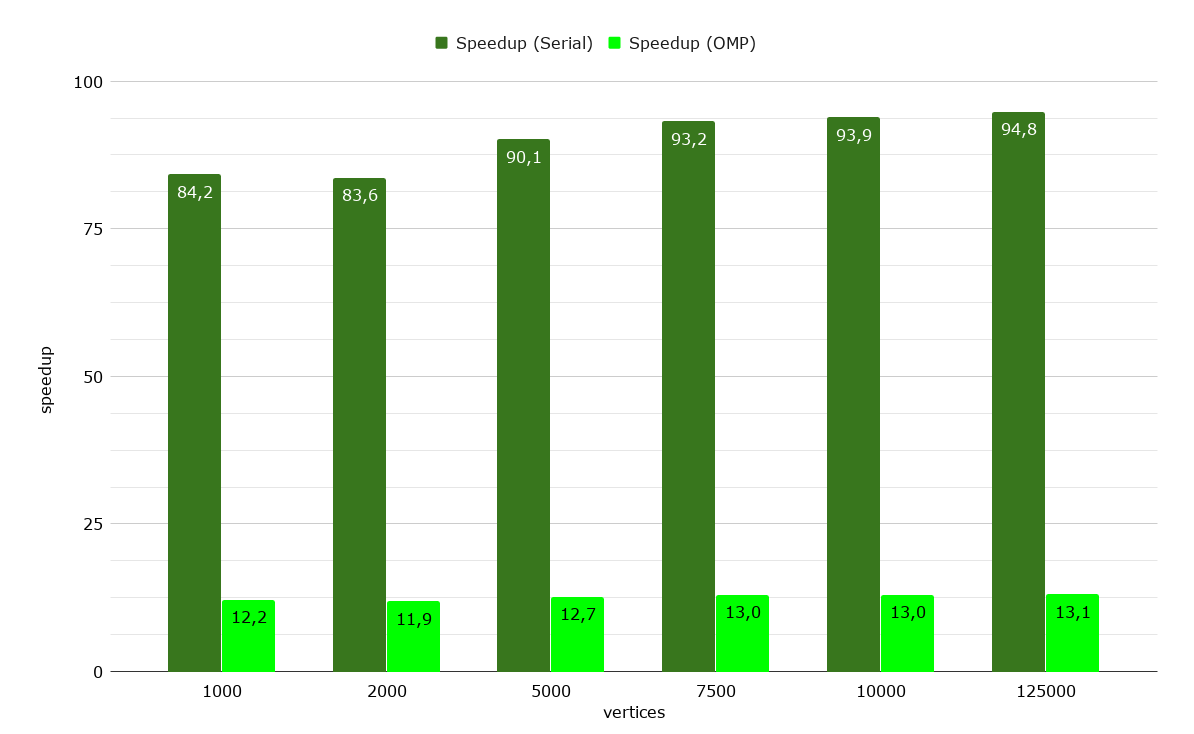
\includegraphics[width=3.5in]{diagrams/cuda-speedup}
\captionsetup{justification=centering}                                                                                                                                   
\caption{Speedup of \emph{CUDA} FW consuming a medium matrix compared to \emph{sequential} and \emph{OMP} FW}                                                                                                                                            
\label{fig:cuda-speedup}                                                                                                                                                           
\end{figure}

Because the CUDA APIs don't allow the user to control the number of Streaming Multiprocessors or how many CUDA cores
can be involved in the computation, the speedup and the efficiency are calculated based on the number of threads per block.


\begin{figure}[h!]
\centering                                                                        
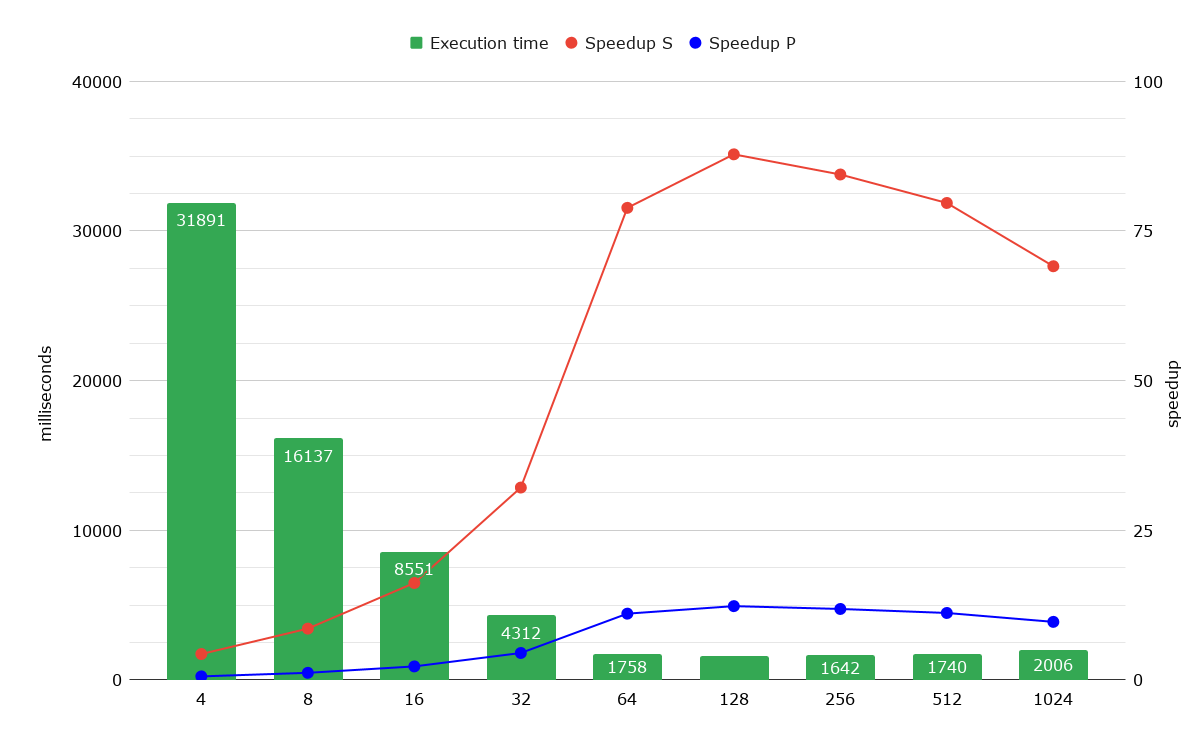
\includegraphics[width=3.5in]{diagrams/cuda-time}
\captionsetup{justification=centering}                                                                                                                                   
\caption{Efficiency of \emph{MPI} FW consuming a medium matrix}                                                                                                                                            
\label{fig:cuda-time}                                                                                                                                                           
\end{figure}






























































\subsection{Hybrid: MPI + OpenMP}
In order to make the most of \emph{MPI FW}, it can be combined with \emph{OpenMP}; this
makes sense because each process runs the $i$ and $j$ for loops with one thread and nowadays
is more than rare to have a cluster composed of single thread CPUs.

\textbf{Algorithm \ref*{alg:mpi+omp}} shows how easily \emph{MPI FW} can be modified
so that each process can benefit from multithreading.
\begin{algorithm}[h!]

\SetAlgoLined

broadcast($n$, $ROOT$) \\
scatter($M$, $processes$)

\texttt{\#pragma omp parallel num\_threads(t) shared(M, k, p)} \\
\For{$k = 1 \rightarrow n$}{
	\texttt{\#pragma omp master} \\
	\If{$rank =$ \textnormal{findOwnerOfKthRow}($k$, $rank$)}{
		$K \leftarrow $ getRow($M$, $k$) \\
		broadcast($K$, $owner$) \\
	}

	\texttt{\#pragma omp for private(i,j) schedule(dynamic)} \\
	\For{$i = 1 \rightarrow \frac{n}{p}$}{
		\For{$j = 1 \rightarrow n$}{
			\If{$M_{i,j} < M_{i,k} + K_j$}{
				$M_{i,j} \leftarrow M_{i,k} + K_j$
			}
		}
	}
}
gather($M$, $processes$);
 
\caption{\emph{MPI+OpenMP} FW}\label{alg:mpi+omp}
\end{algorithm}












\subsection{Hybrid: MPI + CUDA}
\begin{algorithm}[h!]

\SetAlgoLined
\DontPrintSemicolon
broadcast($n$, $ROOT$) \\
scatter($M$, $processes$)

\For{$k = 1 \rightarrow n$}{
	\If{$rank =$ \textnormal{findOwnerOfKthRow}($k$, $rank$)}{
		$K \leftarrow $ getRow($M$, $k$) \\
		broadcast($K$, $owner$) \\
	}

	
  


	\textnormal{kernel<{}<{}<$\frac{n+b-1}{b}$, $b$>{}>{}>($M$, $n$, $k$)}

}
gather($M$, $processes$);
\;
\;
  \SetKwFunction{FMain}{kernel}
  \SetKwProg{Fn}{Function}{:}{}
  \Fn{\FMain{$M$, $n$, $k$}}{


$j \leftarrow \left|B\right|_x \times B_x + T_x$ \\
$i \leftarrow \left|B\right|_y$ \\

\If{$j < n$}{
	

	\If{$M_{i,j} < M_{i,k} + M_{k,j}$}{
		$M_{i,j} \leftarrow M_{i,k} + M_{k,j}$
	}
}
}

 
\caption{\emph{MPI+CUDA} FW}\label{alg:mpi+cuda}
\end{algorithm}


\section{Computational Platforms and Software Libraries}
This section describes technical details about the implementation of the solutions exposed in this document. It also contains
the collected data used for the analysis.

The results of each run are tested with 16bit Fletcher's checksum so that errors can be quickly checked over large matrices \cite{fletcher}.
\subsection{Serial implementation}
The \emph{sequential} version of the FW algorithm can be found \href{https://github.com/firaja/Parallel-FloydWarshall/blob/master/sequential.c}{here}. 
The program compiles as follows:
\begin{lstlisting}[basicstyle=\footnotesize\ttfamily]
$ gcc sequential.c -o sequential.out -O3
\end{lstlisting}

notice the \texttt{-O3} flag that makes the program run $3.5$ times faster.
The program accepts 2 arguments:
\begin{lstlisting}[basicstyle=\footnotesize\ttfamily]
$ ./sequential.out <v> <d>
\end{lstlisting}
where \texttt{v} is the number of verteces, expressed as positive integer, and \texttt{d} is the density of the presence of edges, expressed as an integer from 0 to 100.
\par
The \texttt{gcc} version used for this work is 7.5.0 and the program ran on a Intel Core i7-9700K. \\
\textbf{Table \ref*{tab:seq-time}} shows the execution time (expressed in milliseconds) depending on the number of vertices.


\begin{table}[h!]
\centering
\begin{tabular}{|r|r|}
\hline
\rowcolor[HTML]{3166FF} 
{\color[HTML]{FFFFFF} \textbf{Vertices}} & {\color[HTML]{FFFFFF} \textbf{Execution time}} \\ \hline
1000                                     & 1095 ms                                        \\ \hline
2000                                     & 8860 ms                                        \\ \hline
5000                                     & 138643 ms                                      \\ \hline
7500                                     & 468750 ms                                      \\ \hline
10000                                    & 1112111 ms                                     \\ \hline
12500                                    & 2170138 ms                                     \\ \hline
\end{tabular}
\caption{Execution time of the \emph{serial} FW}                                                                                                                                            
\label{tab:seq-time} 
\end{table}

\textbf{Figure \ref*{fig:seq-time}} shows the trend of the execution time. 

\begin{figure}[h!]
\centering                                                                        
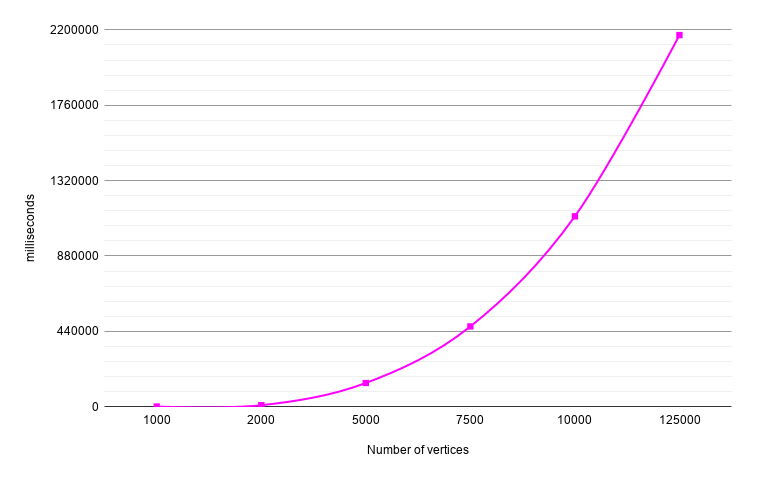
\includegraphics[width=3.5in]{images/seq-time}
\captionsetup{justification=centering,margin=2cm}                                                                                                                                   
\caption{Trend of the execution time based on Table \ref*{tab:seq-time}}                                                                                                                                            
\label{fig:seq-time}                                                                                                                                                           
\end{figure}


It is easy to notice that the graph represents a 
third grade curve; this is the interpolated function starting from the collected data:
\[f(n) = 2.22n^3 - 18.83n^2 + 92.14n -94.84 \in \Theta(n^3) \]



\subsection{MPI implementation}

The \emph{MPI} version of the FW algorithm can be found \href{https://github.com/firaja/Parallel-FloydWarshall/blob/master/mpi.c}{here}. 
The program compiles as it follows:

\begin{lstlisting}[basicstyle=\footnotesize\ttfamily]
$ mpicc -g -Wall mpi.c -o mpi.out -O3
\end{lstlisting}
Like the \emph{serial} version, the program accepts 2 arguments + 1 for $\texttt{mpirun}$:
\begin{lstlisting}[basicstyle=\footnotesize\ttfamily]
$ mpirun -np <p> mpi.out <v> <d>
\end{lstlisting}
The \texttt{MPI} version used for this work is 2.1.1 and the program ran on a cluster of 8 nodes over a LAN. \\
\textbf{Table \ref*{tab:mpi-time}} shows the execution time (expressed in milliseconds) and the percentage of time spent in initialization and communication, depending on the number of processors; 
in this case the program computed the \emph{APSP} problem for 5040 vertices.

\begin{table}[h!]
\centering
\begin{tabular}{|r|r|r|}
\hline
\rowcolor[HTML]{F56B00} 
{\color[HTML]{FFFFFF} \textbf{Processors}} & {\color[HTML]{FFFFFF} \textbf{Execution time}} & {\color[HTML]{FFFFFF} \textbf{MPI \%}} \\ \hline
1                                          & 145447 ms                                               & 0.06                                 \\ \hline
2                                          & 75059 ms                                               & 2.57                                 \\ \hline
3                                          & 52336 ms                                               & 4.45                                \\ \hline
4                                          & 39962 ms                                               & 5.47                                \\ \hline
5                                          & 33184 ms                                               & 6.95                                 \\ \hline
6                                          & 28731 ms                                               & 8.35                                \\ \hline
7                                          & 25853 ms                                               & 9.50                                 \\ \hline
8                                          & 23120 ms                                               & 11.00                                \\ \hline
\end{tabular}
\caption{Execution time of the \emph{MPI} FW}                                                                                                                                            
\label{tab:mpi-time}
\end{table}
Timings are captured through \texttt{mpiP} that calculates the percentage of time spent by MPI for initialization/finalization and communication.
\texttt{mpiP} is a lightweight profiling library for MPI applications. Because it only collects statistical information about MPI functions, \texttt{mpiP} generates considerably less overhead and much less data than tracing tools. All the information captured by mpiP is task-local. It only uses communication during report generation, typically at the end of the experiment, to merge results from all of the tasks into one output file.


\subsection{OpenMP implementation}
The \emph{OpenMP} version of the FW algorithm can be found \href{https://github.com/firaja/Parallel-FloydWarshall/blob/master/openmp.c}{here}. 
The program compiles as it follows:
\begin{lstlisting}[basicstyle=\footnotesize\ttfamily]
$ g++ -fopenmp openmp.c -o openmp.out -O3
\end{lstlisting}
Unlike the \emph{serial} version, the program accepts 3 arguments:
\begin{lstlisting}[basicstyle=\footnotesize\ttfamily]
$ ./openmp.out <v> <d> <t>
\end{lstlisting}
where \texttt{t} is the number of threads OpenMP can use for parallelization. \\
The \texttt{gcc} version used for this work is 7.5.0 and the program ran on a Intel Core i7-9700K, which has 8 core with no Hyper-Threading.
\textbf{Table \ref*{tab:omp-time}} shows the execution time (expressed in milliseconds) depending on the number of vertices and available cores.

\begin{table}[h!]
\centering
\begin{tabular}{|r|r|r|r|}
\hline
\rowcolor[HTML]{CB0000} 
\multicolumn{1}{|c|}{\cellcolor[HTML]{CB0000}{\color[HTML]{FFFFFF} \textbf{Vertices}}} & \multicolumn{1}{c|}{\cellcolor[HTML]{CB0000}{\color[HTML]{FFFFFF} \textbf{2 threads}}} & \multicolumn{1}{c|}{\cellcolor[HTML]{CB0000}{\color[HTML]{FFFFFF} \textbf{4 threads}}} & \multicolumn{1}{c|}{\cellcolor[HTML]{CB0000}{\color[HTML]{FFFFFF} \textbf{8 threads}}} \\ \hline
1000                                                                                   & 541 ms                                                                                         & 364 ms                                                                                         & 158 ms                                                                                          \\ \hline
2000                                                                                   & 4365 ms                                                                                        & 2921 ms                                                                                        & 1260 ms                                                                                         \\ \hline
5000                                                                                   & 69590 ms                                                                                       & 46443 ms                                                                                       & 19496 ms                                                                                        \\ \hline
7500                                                                                   & 230260 ms                                                                                      & 155531 ms                                                                                      & 65118 ms                                                                                        \\ \hline
10000                                                                                  & 543900 ms                                                                                      & 367434 ms                                                                                       & 153682 ms                                                                                       \\ \hline
12500                                                                                  & 1063129 ms                                                                                     & 716363 ms                                                                                       & 299006 ms                                                                                       \\ \hline
\end{tabular}
\caption{Execution time of the \emph{OpenMP} FW}                                                                                                                                            
\label{tab:omp-time}
\end{table}

\subsection{CUDA implementation}
The \emph{CUDA} version of the FW algorithm can be found \href{https://github.com/firaja/Parallel-FloydWarshall/blob/master/cuda.cu}{here} (pre-Volta architecture). Alternatively the version 
that uses only global memory is \href{https://github.com/firaja/Parallel-FloydWarshall/blob/master/cuda2.cu}{here} (Volta and post-Volta architecture).
The program compiles as follows:
\begin{lstlisting}[basicstyle=\footnotesize\ttfamily]
$ nvcc cuda.cu -o cuda.out \
  -gencode=arch=compute_75,code=compute_75 -O3
\end{lstlisting}
Unlike the \emph{serial} version, the program accepts 3 arguments:
\begin{lstlisting}[basicstyle=\footnotesize\ttfamily]
$ ./cuda.out <v> <d> <b>
\end{lstlisting}
where \texttt{b} is the number of threads per block. \\
The \texttt{nvcc} version used for this work is 10.2 and the program ran on a CPU Intel Core i7-9700K and a GPU NVIDIA GeForce RTX 2070 Super.
Table \ref*{tab:cuda-time} shows the execution time (expressed in milliseconds) depending on the number of vertices and the block size of threads.

\begin{table}[h!]
\centering
\begin{tabular}{|r|r|r|r|}
\hline
\rowcolor[HTML]{009901} 
\multicolumn{1}{|l|}{\cellcolor[HTML]{009901}{\color[HTML]{FFFFFF} \textbf{verteces}}} & \multicolumn{1}{l|}{\cellcolor[HTML]{009901}{\color[HTML]{FFFFFF} \textbf{1024 block}}} & {\color[HTML]{FFFFFF} \textbf{256 block}} & \multicolumn{1}{l|}{\cellcolor[HTML]{009901}{\color[HTML]{FFFFFF} \textbf{32 block}}} \\ \hline
1000                                                                                   & 24 ms                                                                                                & 19 ms                                                  & 53 ms                                                                                              \\ \hline
2000                                                                                   & 219 ms                                                                                               & 186 ms                                                 & 356 ms                                                                                            \\ \hline
5000                                                                                   & 2818 ms                                                                                              & 2709 ms                                                & 4966 ms                                                                                            \\ \hline
7500                                                                                   & 9894 ms                                                                                              & 9044 ms                                                & 16297 ms                                                                                           \\ \hline
10000                                                                                  & 22190 ms                                                                                             & 21392 ms                                               & 38208 ms                                                                                           \\ \hline
125000                                                                                 & 42955 ms                                                                                             & 41460 ms                                               & 75034 ms                                                                                           \\ \hline
\end{tabular}
\caption{Execution time of the \emph{CUDA} FW}                                                                                                                                            
\label{tab:cuda-time}
\end{table}


Using a CPU-based timer would measure only the kernel's launch time and not the kernel's execution time and it would require a host-device synchronization point, like \texttt{cudaDeviceSynchronize()} which stalls the GPU pipeline.

So timings are taken with CUDA events that are created and destroyed with \texttt{cudaEventCreate()} and \texttt{cudaEventDestroy()}. \texttt{cudaEventRecord()} places the start and stop events into the default stream  and the device will record a time stamp for the event when it reaches that event in the stream. 
The \texttt{cudaEventElapsedTime()} function returns in the first argument the number of milliseconds time elapsed between the recording events. This value has a resolution of approximately one half microsecond.




\subsection{Hybrid implementation}
The \emph{MPI + OpenMP} version can be found \href{https://github.com/firaja/Parallel-FloydWarshall/blob/master/hybrid.c}{here}. 
The program compiles as follows:
\begin{lstlisting}[basicstyle=\footnotesize\ttfamily]
$ mpicc -g -fopenmp hybrid.c -o hybrid.out -O3
\end{lstlisting}
The program accepts 4 arguments (see $MPI$ and $openMP$ versions):
\begin{lstlisting}[basicstyle=\footnotesize\ttfamily]
$ mpirun -np <p> hybrid.out <n> <d> <t>
\end{lstlisting}





\end{document}

\bibliographystyle{ieeetr}
\bibliography{Bibliography}